\chapter{Drools Concept hierarchy}
\label{appendix:DroolsConceptHierarchy}

The concept hierarchy presented on the following pages was extracted and interpreted from Drools railroad diagrams.

The diagram in figure \ref{fig:RuleFileDiagram} represents the file level and can be considered the root of Concept Hierarchy.
This represents the concepts that are available to the rule file.
As the only concept we will examine in depth is the rule, we show some concepts that are shared or are children of, for example, function, query and type declaration.

In our final implementation only the import, global and Rule concepts that were children of the rule file were implemented.

The diagram in figure \ref{fig:RuleDiagram} shows the children of a rule.
Each attribute has a different behavior and structure and are thus all represented separately.

In These diagrams we do not show a concept diagram for the RHS.
This is because it would be more or less the concept diagram for Java Statements,with the addition of Rule Variables and some special Drools functions.
the concept diagram for a General Purpose Language, like Java, would be orders of magnitude bigger and more complex.
Luckily, as MPS allows for almost seamless extension and integration of different languages, we are able to just import JetBrains implementation of Java for the RHS.

The hierarch for the LHS is shown in the diagram in figure \ref{fig:LHSDiagram}.
Because of the number of concepts being represented, it may be a little hard to read.

\begin{figure}[h]
    \centering
    \fbox{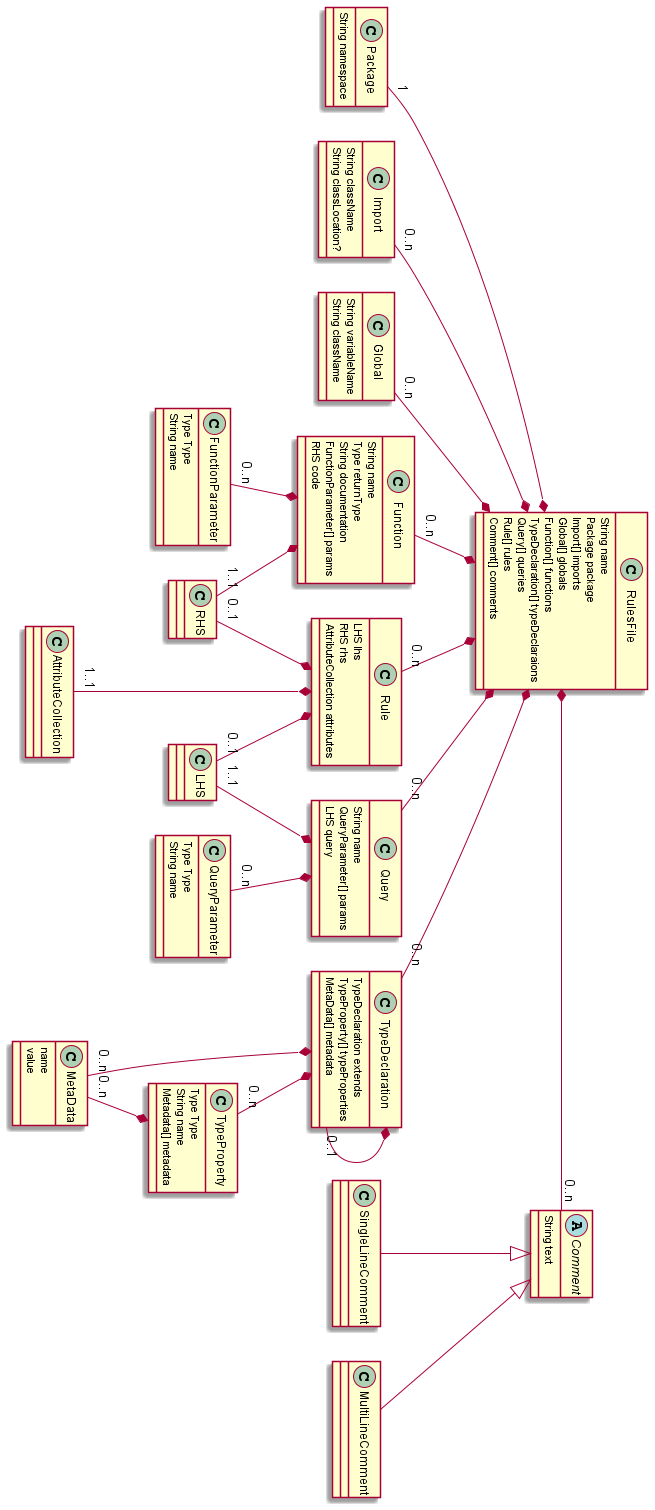
\includegraphics[width=0.75\textwidth]{Appendices/images/Droolsstructurerulefile.png}}
    \caption{Rule file concept hierarchy diagram}
    \label{fig:RuleFileDiagram}
\end{figure}
 

\begin{figure}[h]
    \centering
    \fbox{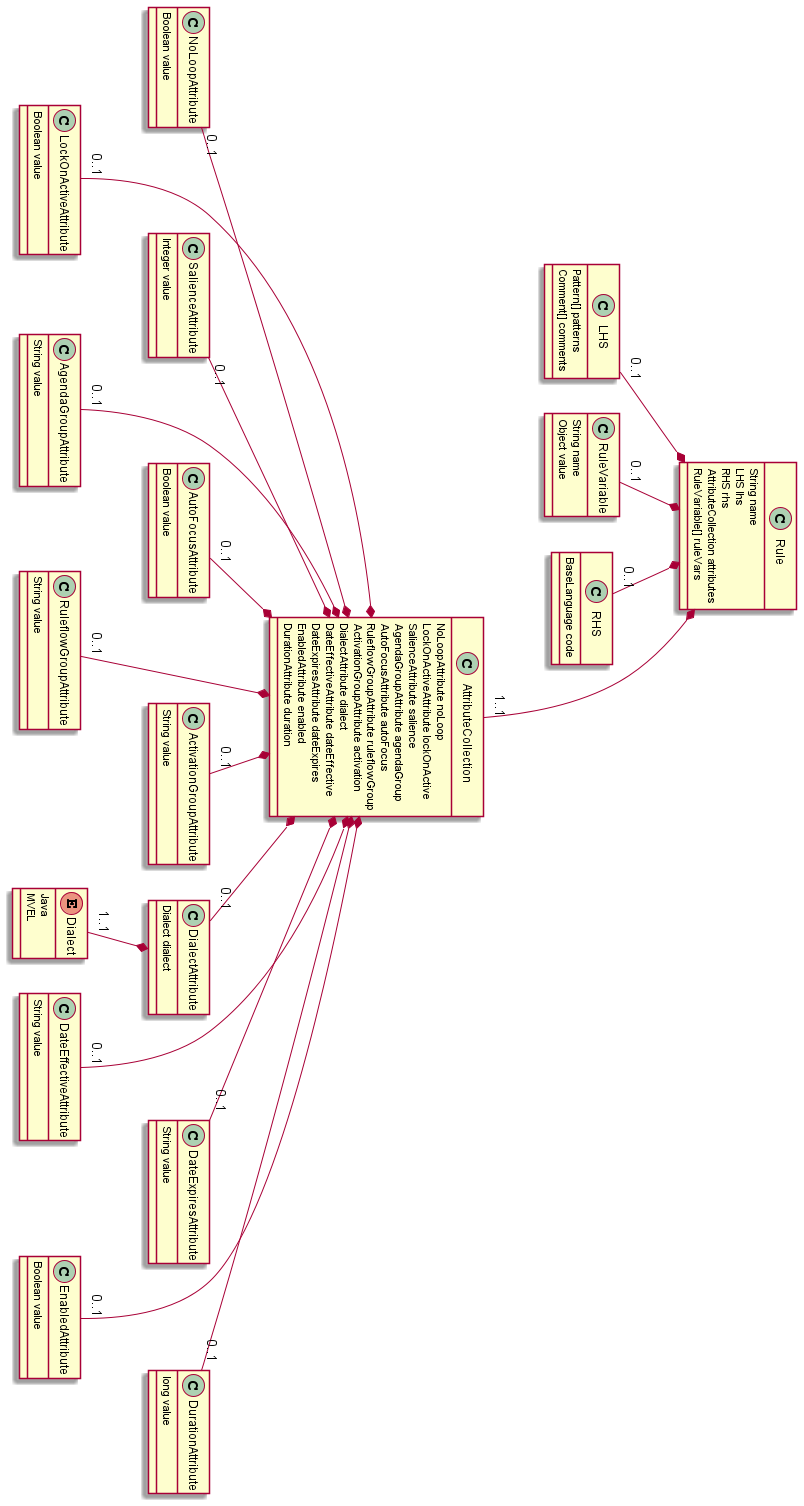
\includegraphics[width=0.95\textwidth]{Appendices/images/Droolsstructurerules.png}}
    \caption{Rules concept hierarchy diagram}
    \label{fig:RuleDiagram}
\end{figure}
 

\begin{figure}[h]
    \centering
    \fbox{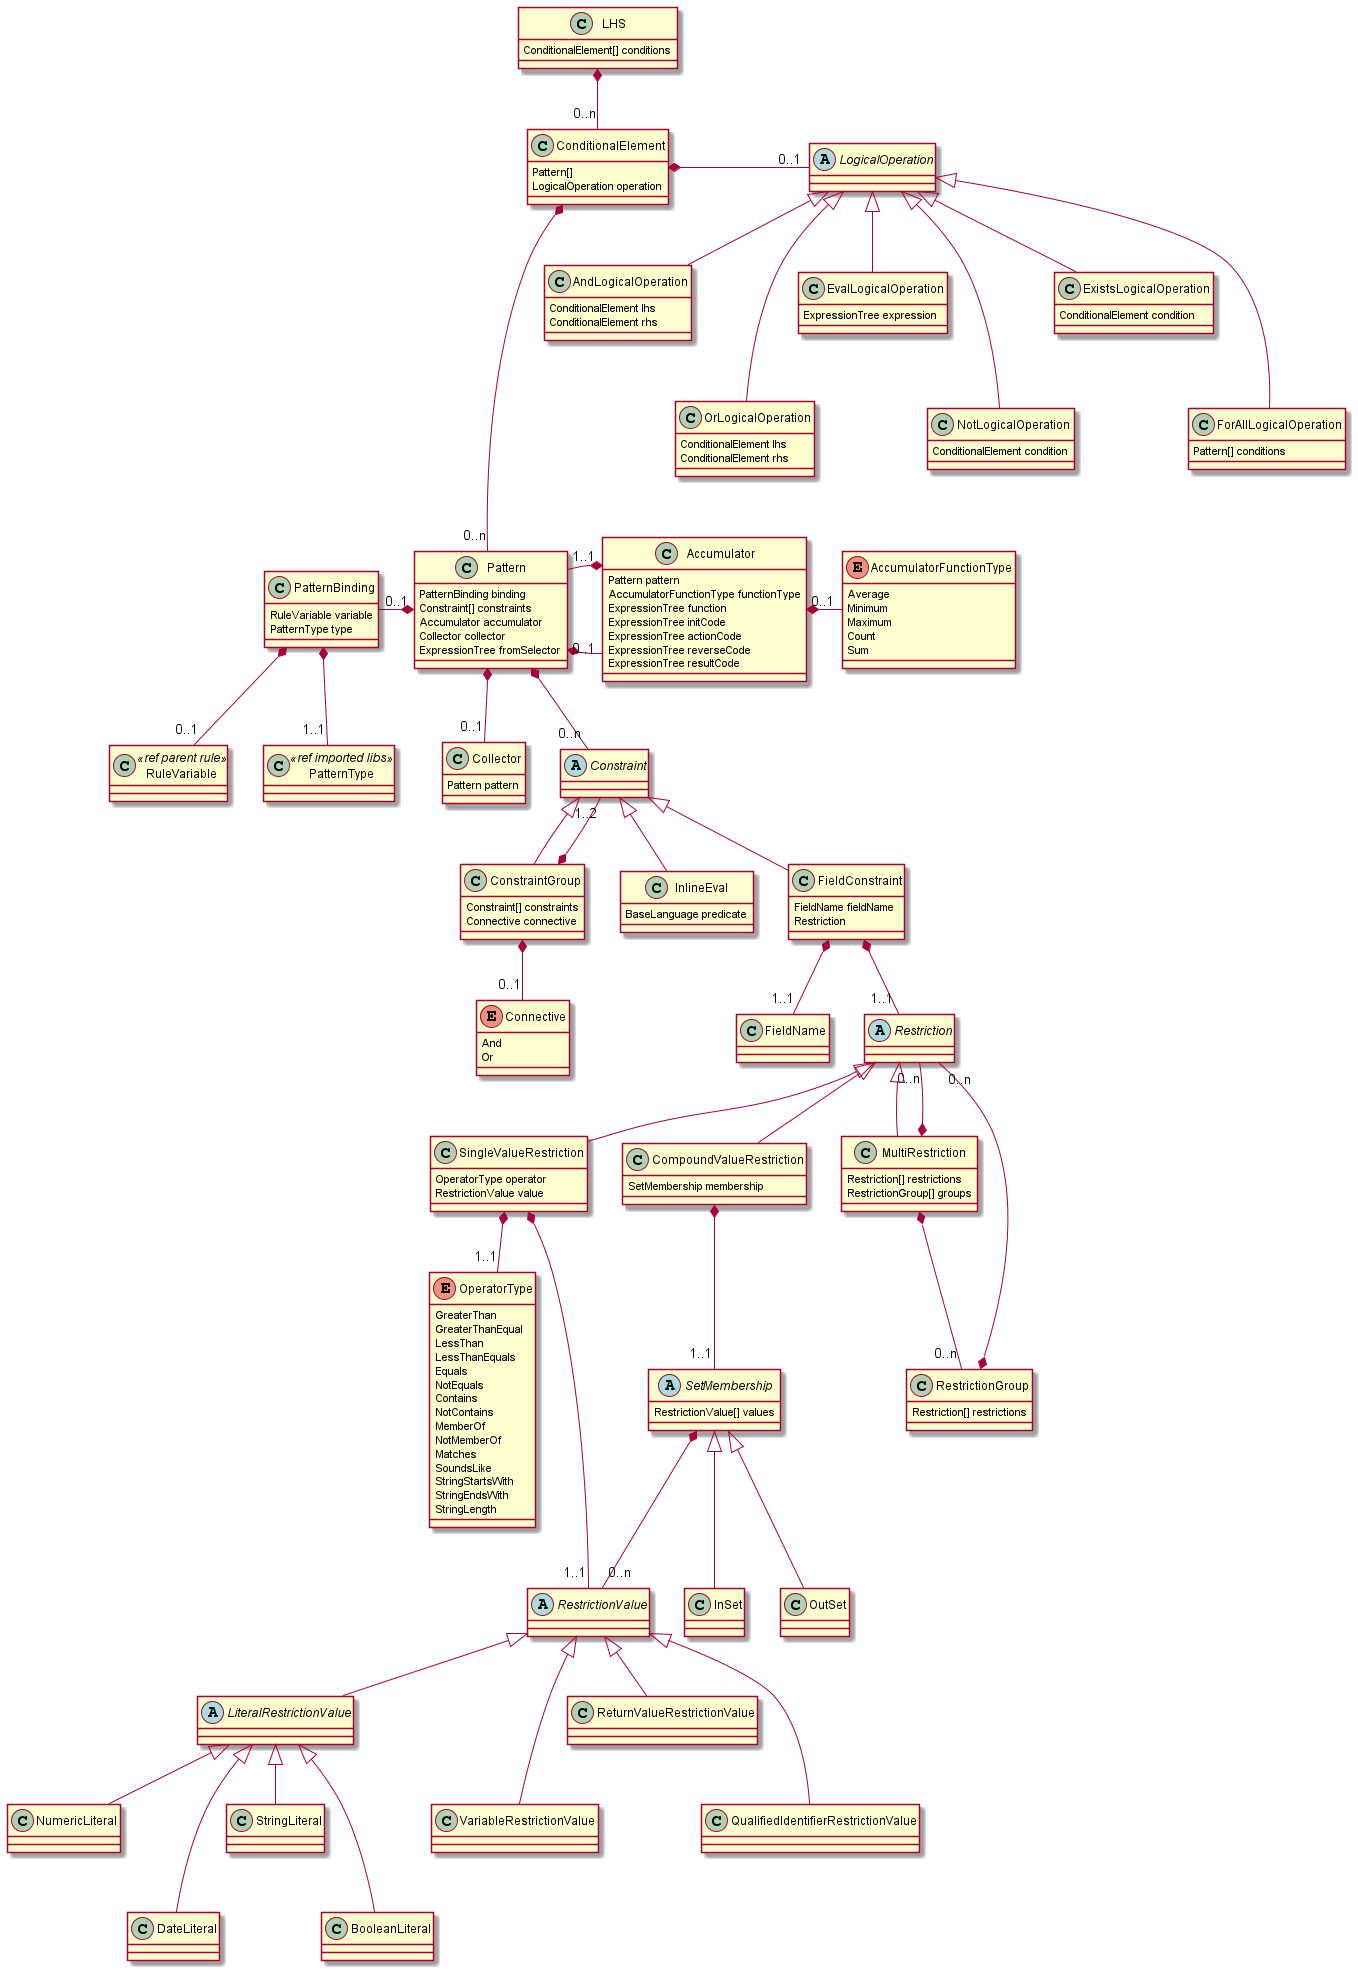
\includegraphics[width=0.99\textwidth]{Appendices/images/DroolsStructureLHS.png}}
    \caption{Rule LHS concept hierarchy diagram}
    \label{fig:LHSDiagram}
\end{figure}
 